\renewcommand{\theequation}{\theenumi}
\begin{enumerate}[label=\thesection.\arabic*.,ref=\thesection.\theenumi]
\numberwithin{equation}{enumi}

\item 
Given,
\begin{align}
    12x^2+7xy-10y^2+13x+45y-35&=0 \label{eq:pair_given}
\end{align}
The above equation \eqref{eq:pair_given} can be expressed as \eqref{eq:conic_quad_form} with
\begin{align}
    \vec{V}=\vec{V}^T&=\myvec{12 & \frac{7}{2}\\\frac{7}{2} &-10}\label{eq:pair_v}\\
    \vec{u}&=\myvec{\frac{13}{2} \\ \frac{45}{2}}\label{eq:pair_u}\\
    f&=-35\label{eq:pair_fv}
\end{align}


shown in equations \eqref{eq:pair_1}, \eqref{eq:pair_2}, \eqref{eq:pair_3}
\begin{align}
    \vec{x}^T\myvec{12 & \frac{7}{2} \\\frac{7}{2} & -10}\vec{x}+2\myvec{\frac{13}{2} & \frac{45}{2}}\vec{x}-35&=0 \label{eq:pair_c}
\end{align}
Comparing equation \eqref{eq:pair_c} with \eqref{eq:pair_1} we get
Substituting the above equations \eqref{eq:pair_v}, \eqref{eq:pair_u}, \eqref{eq:pair_fv} in LHS of equation \eqref{eq:pair_check} to verify the given equation is pair of straight lines
\begin{align}
\delta&=\begin{array}{|ccc|}
12 &\frac{7}{2}& \frac{13}{2}\\\frac{7}{2} & -10 & \frac{45}{2}\\ \frac{13}{2} & \frac{45}{2} & -35
\end{array}&
\intertext{Expanding the above determinant , we get}
\delta&=0
\end{align}
Since equation \eqref{eq:pair_check} is satisfied, we could say that the given equation \eqref{eq:pair_given} represents two straight lines
From equation \eqref{eq:pair_given} 

Consider , 
\begin{align}
    &\hspace{1cm}12x^2+7xy-10y^2\\
    &\implies 12x^2+15xy-8xy-10y^2\\
    &\implies 3x(4x+5y)-2y(4x+5y)\\
    &\implies (3x-2y)(4x+5y)
\end{align}
Therefore equation \eqref{eq:pair_given} can be modified as 
\begin{align}
(3x-2y+l)(4x+5y+m)&=0\label{eq:pair_lines}
\end{align}
\begin{multline}
12x^2 + 7xy -10y^2 + (3m+4l)x\\ 
+(-2m+5l)y+lm=0\label{eq:pair_eq}
\end{multline}
Equating x and y co-efficients of the equations \eqref{eq:pair_given} and \eqref{eq:pair_eq} , we get ,
\begin{align}
    3m+4l&=13\label{eq:pair_lm1}\\
    -2m+5l&=45\label{eq:pair_lm2}
\end{align}
Solving equations \eqref{eq:pair_lm1}, \eqref{eq:pair_lm2} we get ,
\begin{align}
        l&=7\label{eq:pair_l}\\
    m&=-5\label{eq:pair_m}
\end{align}
Substituting the equations \eqref{eq:pair_l}, \eqref{eq:pair_m} in \eqref{eq:pair_lines} we get
\begin{align}
    (3x-2y+7)(4x+5y-5)&=0\label{eq:pair_sl}
\end{align}
The above equation \eqref{eq:pair_sl} represents two straights and straight line equation is given by 
\begin{align}
    3x-2y+7&=0\label{eq:pair_line1}\\
    4x+5y-5&=0\label{eq:pair_line2}
\end{align}

\renewcommand{\thefigure}{1}
\begin{figure}[h]
    \centering
    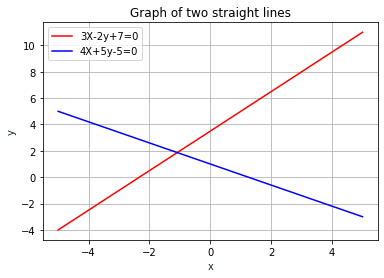
\includegraphics[width=\columnwidth]{./figs/pair/pair_ang.png}
    \caption{Pair of straight lines}
    \label{fig:pair}
\end{figure}

From the straight line equation \eqref{eq:pair_line1}, \eqref{eq:pair_line2} 
\begin{align}
    \vec{n_1}=\myvec{3\\-2}\\
    \vec{n_2}=\myvec{4\\5}
\end{align}
Angle between the two straight lines is given by 
\begin{align}
    \theta&=\cos^{-1}\biggl(\frac{\vec{n_1}^T\vec{n_2}}{\norm{\vec{n_1}}\norm{\vec{n_2}}}\biggr)\label{eq:pair_t}
%\label{eq:pair_theta}
\\
    \vec{n_1}^T\vec{n_2}&=\myvec{3 & -2}\myvec{4\\5}=2\label{eq:pair_tr}\\
    \norm{\vec{n_1}}&=\sqrt{3^2+(-2)^2}=\sqrt{13}\label{eq:pair_norm1}\\
    \norm{\vec{n_2}}&=\sqrt{4^2+5^2}=\sqrt{41}\label{eq:pair_norm2}
\end{align}
Substituting equations \eqref{eq:pair_tr}, \eqref{eq:pair_norm1} ,\eqref{eq:pair_norm2} in equation \eqref{eq:pair_theta}, we get 
\begin{align}
        \theta&=\cos^{-1}\biggl(\frac{2}{\sqrt{13}\sqrt{41}}\biggr)\\
        \theta&=85\degree
\end{align}

$\boldsymbol{ Result : }$

Angle between the two straight line is given by
\begin{align}
    \theta&=85\degree
\end{align}


\end{enumerate}

